\section{Programovacie paradigmy}
\noindent \par
Programovacia paradigma je spôsob riešenia programátorských problémov \cite{samuelInsightProgrammingParadigms2018}.
Poznáme veľké množstvo programovacích paradigiem. Medzi ne patria aj nasledujúce štyri:
\begin{itemize}
  \item Imperatívna paradigma.
  \item Funkcionálna paradigma.
  \item Objektovo orientovaná paradigma.
  \item Udalosťami riadená paradigma.
\end{itemize}

\subsection{Imperatívna paradigma}
\noindent \par
Základnou myšlienkou je príkaz, ktorý má merateľný dopad na aktuálny stav
programu. Pri imperatívnej paradigme je rovnako dôležité aj poradie príkazov. Stav
programu po vykonaní príkazov v ľubovoľnom poradí nemusí byť rovnaký ak by boli príkazy
vykonané v inom poradí \cite{imperativParadigm}.

\subsection{Funkcionálna paradigma}
\noindent \par
Funkcionálna paradigma je postavená na koncepte matematických funkcií, ktoré používajú podmienené
výrazy a rekurziu na vykonanie výpočtu. Zameriava sa na výsledok, nie na spôsobom akým
sa k výsledku dopracovať. Jednou z jeho základných vlastností je nemennosť dát. To
znamená, že ak už bola nejaká štruktúra vytvorená nie je možné meniť jej vnútorný stav.
V prípade potreby zmeny stavu je nutné celú štruktúru vytvoriť odznova. Medzi
najpoužívanejšie funkcionálne jazyky patrí Haskell, Clojure alebo SQL \cite{martinWhatFunctionalProgramming2020}.

\subsection{Objektovo orientovaná paradigma} \label{section:event-driven-programming}
\noindent \par
Paradigma, ktorej myšlienka je inšpirovaná svetom okolo nás. Čokoľvek môže
byť objekt. Auto, dom, kniha či dokument. Každý z týchto objektov má špecifické vlastnosti
a určité správanie. Rovnakým spôsobom modelujeme program. Takéto rozmýšľanie o
objektoch nám umožňuje písať kód, ktorý je jednoduchší na pochopenie a zároveň je
vďaka tomu možné kód rozdeliť na menšie časti. Tieto časti kódu sú následne
jednoduchšie udržiavateľné. Medzi hlavné princípy objektovo orientovaného prístupu
patrí dedičnosť, zapuzdrenosť, polymorfizmus a abstrakcia \cite{Blaschek1994}. Populárne programovacie jazyky podporujúce túto paradigmu sú Python, C\# a Java \cite
{stack-overflow-survey-2020}.

\subsection{Udalosťami riadená paradigma}
\noindent \par
V tejto paradigme je tok programu určený udalosťami. Udalosti môžu byť
rôzne. Väčšinou sa generujú pri akciách používateľa. Príkladom môže byť stlačenie tlačidla
alebo písanie na klávesnici. Udalosti môžu byť generované aj rôznymi perifériami systému ako napríklad pomocou senzorov alebo komunikačnými protokolmi. Niekedy môže byť udalosť generovaná interne, napríklad časovačom alebo prerušením. Bez ohľadu na
zdroj alebo typ udalostí, udalosťami riadené programovanie
hovorí o programovacej paradigme, v ktorej sa tok
programu určuje udalosťami.
\par V dnešnej dobe je možné použiť akýkoľvek programovací jazyk na implementáciu tejto paradigmy. Implementácia by mala zahŕňať nasledujúce časti:
\begin{enumerate}
  \item Zachytávanie udalostí
\end{enumerate}

\noindent \par
Táto časť programu je zodpovedná za zachytávanie vygenerovaných udalostí, ich identifikáciu a prípadné predspracovanie udalosti.

\begin{enumerate}[resume]
  \item Rozposielanie udalostí
\end{enumerate}

\noindent \par
Po zachytení udalosti nasleduje jej rozposlanie. V tejto časti program identifikuje obsluhy udalostí, ktoré je potrebné vyvolať na základe typu udalosti. Ak daný typ udalosti nemá zaregistrovanú žiadnu obslužnú funkciu, program buď udalosť odignoruje alebo vygeneruje výnimku.

\begin{enumerate}[resume]
  \item Obsluha udalostí
\end{enumerate}

\noindent \par
Časť programu, ktorá je zodpovedná za konečnú obsluhu udalosti. Tu sa nachádza kód, ktorý vykonáva potrebnú funkcionalitu. Ako príklad môžeme uviesť stlačenie tlačidla na klávesnici v textovom editore. Po stlačení sa práve tu nachádza logika programu, ktorá zabezpečí vykreslenie písmena na obrazovku.

\begin{figure}[!htbp]
  \centering
  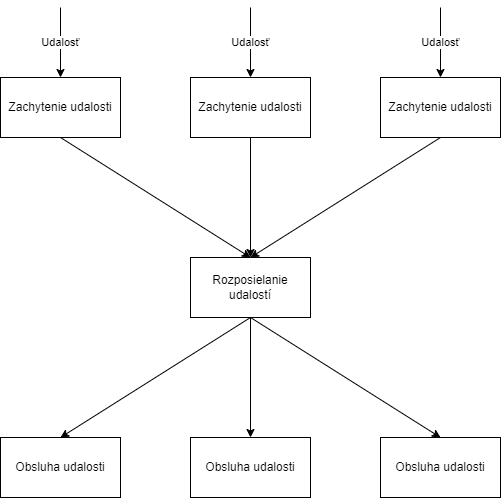
\includegraphics[width=0.60\textwidth]{img/event-driven-schema.png}
  \caption{Schéma implementácie udalosťami riadeného programovania}
  \source{\cite{dashEventDrivenProgramming2011}}
  \label{figure:event-driven-schema}
\end{figure}

\par
Udalosťami riadené programy je možné rozdeliť na dva typy. Prvým typom sú programy, ktoré si neuchovávajú aktuálny stav v ktorom sa nachádzajú. To znamená, že pri obsluhe udalosti vykonajú vždy rovnakú aktivitu bez ohľadu na to aké udalosti nastali v minulosti. Druhým typom sú programy, kde tok vykonávania závisí nielen od aktuálnej udalosti, ale aj sledu predchádzajúcich udalostí \cite{dashEventDrivenProgramming2011}.
\par Táto diplomová práca sa venuje práve týmto druhým typom udalosťami riadených programov a ich modelovaniu pomocou deterministických konečných automatov.